\documentclass{beamer}
\usetheme{AnnArbor}
% \usecolortheme{default}
\usecolortheme{beaver} % Change color theme to red
% Title Page
\title[Short Title]{Tight Frames and Matroids}
\author{Kai Chun Lin}
\institute{Rose-Hulman Institute of Technology}
\usepackage{amsmath,amssymb,amsthm}
\newcommand{\RR}{\mathbb{R}}

\usepackage{tikz, pgfplots}
\usetikzlibrary{arrows, calc}
\pgfplotsset{compat=1.18}

\usepackage{mathtools}
\DeclarePairedDelimiter\set{\{}{\}}
\usepackage{multicol}
\usepackage{biblatex}
\addbibresource{library.bib}

\renewcommand{\vec}[1]{\mathbf{#1}}
\newcommand{\ivec}[2][.8]{%
  \scalebox{#1}{%
    \renewcommand{\arraystretch}{.8}%
    $\begin{bmatrix}#2\end{bmatrix}$%
  }
}
\usebackgroundtemplate{
\ifnum\thepage=1
    \begin{tikzpicture}[overlay, remember picture]
      \node[anchor=north east, inner sep=0pt] at ([xshift = -96pt,yshift=7pt]current page.north east) {\includegraphics[width=6cm]{Photo/Rose+Hulman+Logo.png}};
    \end{tikzpicture}
    \else
  \begin{tikzpicture}[overlay, remember picture]
    \node[anchor=north east, inner sep=17pt] at ([xshift=65pt]current page.north east) {\includegraphics[width=6cm]{Photo/Rose+Hulman+Logo.png}};
  \end{tikzpicture}
  \fi
}
\setbeamercolor{title page}{fg=black,bg=red}
\date{ March 10, 2024}

\begin{document}

\begin{frame}
  \titlepage
\end{frame}

% Outline
\begin{frame}{Outline}
  \tableofcontents
\end{frame}

% % Sample Slide
% \section{Introduction}
% \begin{frame}{Introduction}
%   \begin{itemize}
%     \item Brief overview of the topic
%     \item Objectives of the presentation
%   \end{itemize}
% \end{frame}

% Main Content
\section{Introduction of Matroid, Frame and Tight Frame}
\begin{frame}{Introduction of Matroid}
 \begin{itemize}
    \item Matroid is a generalization of linearly independent set
    % \item A finite matroid $M$ is a pair $(E, \mathcal{I})$, where E is a finite set\\
    % (referred to as the ground set) and $\mathcal{I}$ is a collection of subsets of $E$ (referred to as the independent sets), satisfying the three axioms.
    % \cite{datta2019low}
    \item A \textbf{matroid} is a pair $(S,I)$ with $S$ being a \textbf{ground set} and $I$ is a collection of subsets of $S$ such that it satisfy this 3 axioms
     \item Axioms
     
      \begin{enumerate}
      
        \item The empty set is independent $\emptyset \in \textit{I}$
        \item Every subset of an independent set is independent
        \item If If $A$ and $B$ are two independent sets (i.e., each set is independent) and $A$ has more elements than $B$, then there exists $x \in A \setminus B$ such that $B \cup \{x\}$ is in $\mathcal{I}$.
        \cite{oxley2003matroid}
    \end{enumerate}
  \end{itemize}
\end{frame}

\begin{frame}{Introduction of  Graphic Matroid}
\begin{figure}
  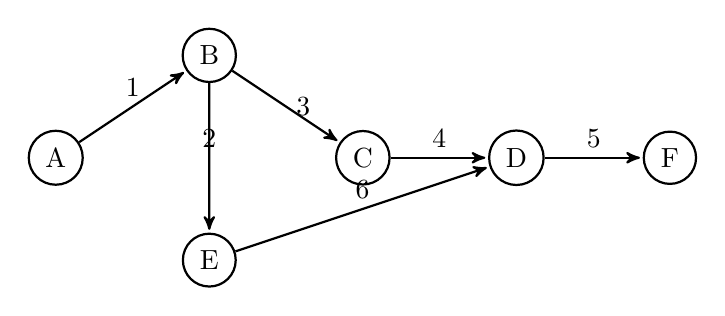
\begin{tikzpicture}[->,>=stealth',shorten >=1pt,auto,node distance=3cm,thick,scale=0.65]
  % Define nodes
  \node[circle, draw] (A) at (0,0) {A};
  \node[circle, draw] (B) at (3,2) {B};
  \node[circle, draw] (C) at (6,0) {C};
  \node[circle, draw] (D) at (9,0) {D};
  \node[circle, draw] (E) at (3,-2) {E};
  \node[circle, draw] (F) at (12,0) {F};
  
  % Draw edges with labels
  \draw (A) edge node[above] {1} (B);
  \draw (B) edge node[above] {2} (E);
  \draw (B) edge node[right] {3} (C);
  \draw (C) edge node[above] {4} (D);
  \draw (E) edge node[above] {6} (D);
  \draw (D) edge node[above] {5} (F);
\end{tikzpicture}
\caption{Caption?}
\end{figure}
\begin{itemize}
    \item <1-> Simple graphs such as this define \textit{graphic matroids}.
    \item <2-> Dependent sets are sets of edges that contain circuits.
\end{itemize}
\end{frame}
\begin{frame}{Introduction to Graphic Matroid}
    
    \begin{itemize}
       \item In this graph the \textbf{groundset} $S =\{1,2,3,4,5,6\}$ and \textit{maximal} independent sets are
       \[
            I = \{\{1, 2, 3, 5, 6\}, \{1, 3, 4, 5, 6\}, ...\}
       \]
    %    \[I = \{ \begin{aligned}
    %     &\emptyset , \{1\} , \{2\} , \dots ,\{6\} ,
    % \{1,2\} , \{1,3\}, \dots \\
    %   &\{1,3,2,6,5\} , \{1,3,4,6,5\} ,\{1,2,6,4,5\} , \{1,2,3,4,5\}
    % \}
    % \end{aligned}\]
        \item Independent sets are collections without cycles why?
        \item Example of Independent set $\{1,2,3,5\} , \{3,2,1\}$
        \item Example of Dependent set $\{2,3,4,6\}$
        
    \end{itemize}
    Does anyone know what is the example of dependent set?

\end{frame}
\begin{frame}{Introduction to Graphic Matroid}
    \begin{itemize}
        \item A \textbf{maximal} independent set is called a \textbf{base}.
        \item Every \textbf{base} of a given matroid has the same size.
        why?
        \item Can you think some examples of base for the previous graph?
        \item $\{1,3,2,6,5\} , \{1,3,4,6,5\} , \{1,2,6,4,5\}$ these are bases of the graph.
        \item The \textbf{rank} of a matroid is the size of any base.
        \item A \textbf{circuit} is a minimal dependent set.
    \end{itemize}
\end{frame}
\begin{frame}{Example of Matroid}
    \[A = \begin{bmatrix}
    1 & 0 & 0 & 1 & 1 & 0 \\
    0 & 1 & 0 & 1 & 0 & 1 \\
    0 & 0 & 1 & 0 & 1 & 1
    \end{bmatrix}\]
    \[E = \{1,2,3,4,5,6 \}\]

    \begin{itemize}
        \item <1-> Independent sets are
        \[
        \{\emptyset, \{1\}, \{2\}, \{3\}, \{1,2\}, \{1, 3\}, \{2, 3\}, \{1, 2, 3\}\}.
        \]
    \end{itemize}
\end{frame}

\begin{frame}{Application of Matroid}

%     \item Matroids seem very mathematical, but they can model many real problems. Many graph
% theory problems can be restated in matroid language using the construction above, and the
% restatement of famous graph algorithms – Kruskal’s minimum weight spanning tree or finding
% a matching in a graph – have very natural interpretations. Similarly, we can (and do!) go
% the other way. Proving statements for matroids also proves them for all the objects matroids
% generalize, and this is a very powerful tool in mathematics
\begin{itemize}
    \item <1->
    \item <2->
    \item <3->
\end{itemize}
    
\end{frame}


\begin{frame}{Introduction of Frame}
  \begin{itemize}
    % \item Frames are collections of vectors that can approximate any vector in the space with arbitrary accuracy, allowing for redundancy in representation.
    
    \item In linear algebra, a frame of an inner product space is a generalization of a basis of a vector space to sets that may be linearly dependent.\cite{kovavcevic2008introduction}
    
    \item In finite-dimensional vector spaces, frames are spanning sets.
    %Frame_Motion_Signal_Processing
    \item In the signal processing, a frame provides a redundant, stable way of representing a signal.\cite{goyal2001quantized}
    
  \end{itemize}
\end{frame}

\begin{frame}{Application of Frame}
  \begin{itemize}
    % \item Frames are used in error detection and correction and the design and analysis of filter banks and more generally in applied mathematics, computer science, and engineering.

  \item \textbf{Signal Processing}
  % : Frames are used for signal denoising, compression, and reconstruction. They provide a flexible framework for representing signals in various domains, such as time, frequency, or spatial.
  
  \item \textbf{Image Processing}
  % : Frames are employed for image compression, enhancement, and restoration. They enable efficient representation of image patches and facilitate robust image reconstruction from incomplete or noisy data.
  
  \item \textbf{Data Compression}
  % : Frames play a crucial role in data compression techniques, such as JPEG and MP3. By exploiting the redundancy inherent in signals or images, frames allow for efficient encoding and decoding processes.
  
  \item \textbf{Sensing and Sampling}
  % : Frames are utilized in sensor networks and sampling schemes for signal acquisition and reconstruction. They enable the design of sampling matrices that satisfy specific sensing or recovery properties.
  
  \item \textbf{Communications}
  % : Frames are used in communication systems for channel coding, modulation, and equalization. They enable reliable transmission of information over noisy or bandwidth-limited channels.
  \end{itemize}
\end{frame}

\begin{frame}{Example of Frame}
  \begin{itemize}
    \item 
    \item 
    \item 
  \end{itemize}
\end{frame}

\begin{frame}
    \frametitle{Bases and erasures}
    \begin{multicols}{2}
        \begin{itemize}
            \item <1-> Let $\set{\vec{e}_{i}}_{i=1}^{2}$ denote the (orthonormal) basis given by $\vec{e}_{1} = \ivec{1\\0},\vec{e}_{2} = \ivec{0\\1}$.
            Let $\vec{x} = 2\vec{e}_{1}+3\vec{e}_{2}$.
            
            \item <2-> If sender transmits $2,3$ successfully to receiver, then $\vec{x}$ can be reconstructed.

            \item <3-> Suppose only $2$ is successfully transmitted. 
            Receiver then constructs the vector $\hat{\vec{x}} = \ivec{2\\0}$.

        \end{itemize}
        \columnbreak
        \only<1>{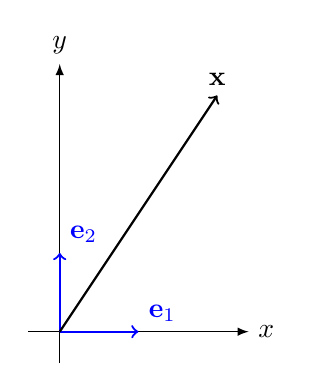
\begin{tikzpicture}
            \coordinate (O)   at (0,0);
            \coordinate (XAxisMin) at (-.4,0);
            \coordinate (XAxisMax) at (2.4,0);
            \coordinate (YAxisMin) at (0,-.4);
            \coordinate (YAxisMax) at (0,3.4);
            \draw [thin, black,-latex] (XAxisMin) -- (XAxisMax) node[right] {$x$};% Draw x axis
            \draw [thin, black,-latex] (YAxisMin) -- (YAxisMax) node[above] {$y$};% Draw y axis
    
            \draw[blue, thick, ->] (O)--(1,0) node[above right] {$\vec{e}_{1}$};
            \draw[blue, thick, ->] (O)--(0,1) node[above right] {$\vec{e}_{2}$};
    
            % \draw[blue, thick, ->] (O)--(1,0) node[above right] {$\vec{e}_{1}$};
            % \draw[blue, thick, ->] (O)--(0,1) node[above right] {$\vec{e}_{2}$};

            % \node at (2,3) {$\bullet$};
            \draw[black, thick, ->] (O)--(2,3) node[above] {$\vec{x}$};
        \end{tikzpicture}}
        \only<2>{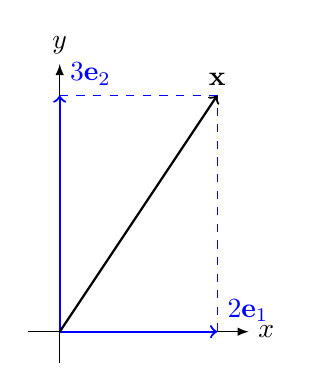
\begin{tikzpicture}
            \coordinate (O)   at (0,0);
            \coordinate (XAxisMin) at (-.4,0);
            \coordinate (XAxisMax) at (2.4,0);
            \coordinate (YAxisMin) at (0,-.4);
            \coordinate (YAxisMax) at (0,3.4);
            \draw [thin, black,-latex] (XAxisMin) -- (XAxisMax) node[right] {$x$};% Draw x axis
            \draw [thin, black,-latex] (YAxisMin) -- (YAxisMax) node[above] {$y$};% Draw y axis
    
            % \draw[blue, ultra thick, ->] (O)--(1,0) node[above right] {$\vec{e}_{1}$};
            % \draw[blue, ultra thick, ->] (O)--(0,1) node[above right] {$\vec{e}_{2}$};
    
            \draw[blue, thick, ->] (O)--(2,0) node[above right] {$2\vec{e}_{1}$};
            \draw[blue, thick, ->] (O)--(0,3) node[above right] {$3\vec{e}_{2}$};
            \draw[blue, dashed] (2,0)--(2,3);
            \draw[blue, dashed] (0,3)--(2,3);
            % \node at (2,3) {$\bullet$};
            \draw[black, thick, ->] (O)--(2,3) node[above] {$\vec{x}$};
        \end{tikzpicture}}
        \only<3->{\begin{tikzpicture}
            \coordinate (O)   at (0,0);
            \coordinate (XAxisMin) at (-.4,0);
            \coordinate (XAxisMax) at (2.4,0);
            \coordinate (YAxisMin) at (0,-.4);
            \coordinate (YAxisMax) at (0,3.4);
            \draw [thin, black,-latex] (XAxisMin) -- (XAxisMax) node[right] {$x$};% Draw x axis
            \draw [thin, black,-latex] (YAxisMin) -- (YAxisMax) node[above] {$y$};% Draw y axis
    
            % \draw[blue, ultra thick, ->] (O)--(1,0) node[above right] {$\vec{e}_{1}$};
            % \draw[blue, ultra thick, ->] (O)--(0,1) node[above right] {$\vec{e}_{2}$};
    
            % \draw[blue, thick, ->] (O)--(2,0) node[above right] {$2\vec{e}_{1}$};
            % \draw[blue, thick, ->] (O)--(0,3) node[above right] {$3\vec{e}_{2}$};
            % \draw[blue, dashed] (2,0)--(2,3);
            % \draw[blue, dashed] (0,3)--(2,3);
            % \node at (2,0) {$\bullet$};
            \draw[black, thick, ->] (O)--(2,3) node[above] {$\vec{x}$};
            \draw[red, thick, ->] (O)--(2,0) node[above] {$\hat{\vec{x}}$};
        \end{tikzpicture}}
    \end{multicols}
    \begin{itemize}
        \item <4-> Impossible to accurately reconstruct $\vec{x}$ if a (nonzero) coefficient is lost!
        Problem is that a basis has no redundancy.
    \end{itemize}
\end{frame}

\begin{frame}
    \frametitle{Frames and erasures}
    \begin{multicols}{2}
        \begin{itemize}
            \item <1-> Let 
            \[
                \vec{f}_{1} = \ivec{0\\1},\vec{f}_{2} = \ivec{-\frac{\sqrt{3}}{2} \\ -\frac{1}{2}}, \vec{f}_{3} = \ivec{\frac{\sqrt{3}}{2} \\ -\frac{1}{2}}.
            \]
            $\set{\vec{f}_{i}}_{i=1}^{3}$ is a frame for $\RR^{2}$.
            
            \item <2-> Let $\vec{x} = \ivec{2\\3}$.
            Then $\vec{x} = 2\vec{f}_{1} - (\frac{2}{\sqrt{3}} + 1)\vec{f}_{2} + (\frac{2}{\sqrt{3}} - 1)\vec{f}_{3}$.

            \item <3-> Suppose only $2$ and $-(\frac{2}{\sqrt{3}}+1)$ are successfully transmitted. 
            Receiver then constructs the vector $\hat{\vec{x}} = 2\vec{f}_{1} - (\frac{2}{\sqrt{3}} + 1)\vec{f}_{2}$.

        \end{itemize}
        \columnbreak
        \only<1>{\begin{tikzpicture}
            \coordinate (O)   at (0,0);
            \coordinate (XAxisMin) at (-1.4,0);
            \coordinate (XAxisMax) at (2.4,0);
            \coordinate (YAxisMin) at (0,-.4);
            \coordinate (YAxisMax) at (0,3.4);

            \draw [thin, black,-latex] (XAxisMin) -- (XAxisMax) node[right] {$x$};% Draw x axis
            \draw [thin, black,-latex] (YAxisMin) -- (YAxisMax) node[above] {$y$};% Draw y axis
            \draw[blue, thick, ->] (O)--(0,1) node[above right] {$\vec{f}_{1}$};
            \draw[blue, thick, ->] (O)--(-{sqrt(3)/2},-1/2) node[left] {$\vec{f}_{2}$};
            \draw[blue, thick, ->] (O)--({sqrt(3)/2},-1/2) node[right] {$\vec{f}_{3}$};
        \end{tikzpicture}}
        \only<2>{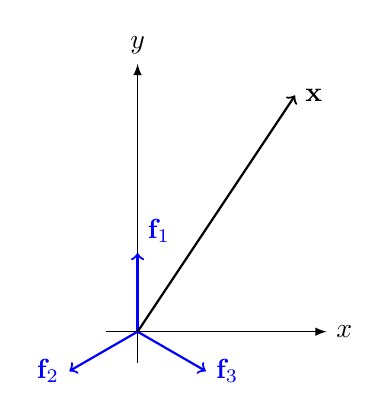
\begin{tikzpicture}
            \coordinate (O)   at (0,0);
            \coordinate (XAxisMin) at (-.4,0);
            \coordinate (XAxisMax) at (2.4,0);
            \coordinate (YAxisMin) at (0,-.4);
            \coordinate (YAxisMax) at (0,3.4);
            \draw [thin, black,-latex] (XAxisMin) -- (XAxisMax) node[right] {$x$};% Draw x axis
            \draw [thin, black,-latex] (YAxisMin) -- (YAxisMax) node[above] {$y$};% Draw y axis
    
            \draw[blue, thick, ->] (O)--(0,1) node[above right] {$\vec{f}_{1}$};
            \draw[blue, thick, ->] (O)--(-{sqrt(3)/2},-1/2) node[left] {$\vec{f}_{2}$};
            \draw[blue, thick, ->] (O)--({sqrt(3)/2},-1/2) node[right] {$\vec{f}_{3}$};
            \draw[black, thick, ->] (O)--(2,3) node[right] {$\vec{x}$};
        \end{tikzpicture}}
        \only<3->{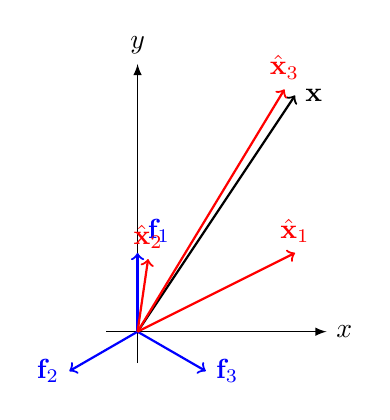
\begin{tikzpicture}
            \coordinate (O)   at (0,0);
            \coordinate (XAxisMin) at (-.4,0);
            \coordinate (XAxisMax) at (2.4,0);
            \coordinate (YAxisMin) at (0,-.4);
            \coordinate (YAxisMax) at (0,3.4);

            \coordinate (f1) at (0,1);
            \coordinate (f2) at (-{sqrt(3)/2},-1/2);
            \coordinate (f3) at ({sqrt(3)/2},-1/2);
            \coordinate (Xhat3) at ($2*(f1)-{2/sqrt(3)}*(f2)-(f2)$);
            \coordinate (Xhat1) at ($-{2/sqrt(3)}*(f2)-(f2) + {2/sqrt(3)}*(f3)-(f3)$);
            \coordinate (Xhat2) at ($(f1) + {2/sqrt(3)}*(f3)-(f3)$);
            % \coordinate (Yhat) at ($2*(f1)+{2/sqrt(3)}*(f3)-(f3)$);
            % \coordinate (Zhat) at ($-{2/sqrt(3)}*(f2)-(f2)+{2/sqrt(3)}*(f3)-(f3)$);
            \draw [thin, black,-latex] (XAxisMin) -- (XAxisMax) node[right] {$x$};% Draw x axis
            \draw [thin, black,-latex] (YAxisMin) -- (YAxisMax) node[above] {$y$};% Draw y axis
    
            % \draw[blue, ultra thick, ->] (O)--(1,0) node[above right] {$\vec{e}_{1}$};
            % \draw[blue, ultra thick, ->] (O)--(0,1) node[above right] {$\vec{e}_{2}$};
    
            % \draw[blue, thick, ->] (O)--(2,0) node[above right] {$2\vec{e}_{1}$};
            % \draw[blue, thick, ->] (O)--(0,3) node[above right] {$3\vec{e}_{2}$};
            % \draw[blue, dashed] (2,0)--(2,3);
            % \draw[blue, dashed] (0,3)--(2,3);
            % \node at (2,0) {$\bullet$};
            \draw[blue, thick, ->] (O)--(0,1) node[above right] {$\vec{f}_{1}$};
            \draw[blue, thick, ->] (O)--(-{sqrt(3)/2},-1/2) node[left] {$\vec{f}_{2}$};
            \draw[blue, thick, ->] (O)--({sqrt(3)/2},-1/2) node[right] {$\vec{f}_{3}$};
            \draw[black, thick, ->] (O)--(2,3) node[right] {$\vec{x}$};
            \draw[red, thick, ->] (O)--(Xhat3) node[above] {$\hat{\vec{x}}_3$};
            \draw[red, thick, ->] (O)--(Xhat1) node[above] {$\hat{\vec{x}}_1$};
            \draw[red, thick, ->] (O)--(Xhat2) node[above] {$\hat{\vec{x}}_2$};
            % \draw[red, thick, ->] (O)--(Yhat) node[above] {$\hat{\vec{y}}$};
            % \draw[red, thick, ->] (O)--(Zhat) node[above] {$\hat{\vec{z}}$};
        \end{tikzpicture}}
    \end{multicols}
\end{frame}

\begin{frame}{Some important theorems}
    \begin{theorem}[K. Lin, 2023]
%A $(d+1, d)$ ETF can be constructed by first constructing a corresponding Gram matrix $G$ using the formula
Given the $(d+1, d)$ ETF with Gram matrix
$G = \frac{d+1}{d}I_{d+1} -\frac{1}{d}J$,
%Then we need to add together columns of this matrix taken k at a time to form the particular matroid.
form a collection of $\binom{d+1}{d} = d+1$ vectors by adding together $d$ vectors from the ETF at a time.
The matroid corresponding to this new collection has only one circuit, namely, the set $\{1, 2, \ldots, d, d+1\}$.
% We found that if $k=d$ this matroid has only one circuit.
\end{theorem}
\begin{proof}
% Since in the case $k=d$. In the first, we will have $k+1$ vector and to pick $d$ vectors and add them together to get a new vector and add this new vector in the matroid.
Since $\sum_{i=1}^{d+1}\vec{f}_i = \vec{0}$,
if we pick $d$ vectors at a time is equivalent to picking $(d+1)-d = 1$ vector at a time. 
Then, if $d=k$ which means to pick one vector at the time and add the vector to the matrix which did not add anything to the matroid.
Accordingly, if $k=d$ this matroid has only one circuit which is $\{1, 2, \ldots, d, d+1\}$.
In other word, every columns is a dependent set but if we remove any columns it will be independent set.
\end{proof}
\end{frame}


\begin{frame}{Introduction of Tight Frame}
  \begin{itemize}
    \item 
    \item 
    \item 
  \end{itemize}
\end{frame}

\begin{frame}{Example of Tight Frame}
  \begin{itemize}
    \item 
    \item 
    \item 
  \end{itemize}
\end{frame}

\begin{frame}{Application of Tight Frame}
  \begin{itemize}
    \item 
    \item 
    \item 
  \end{itemize}
\end{frame}


%Research Result
\section{Research result}
\begin{frame}{Theorem 1}
  \begin{itemize}
    \item 
    \item 
    \item 
  \end{itemize}
\end{frame}

% Conclusion
\section{Conclusion}
\begin{frame}{Acknowledgements}
    This work was supported by the SURE.2020.WV.03 SURE Grant through the WV Research Challenge Fund, WV Higher Education Policy Commission.
\end{frame}
\begin{frame}{Conclusion}
  \begin{itemize}
    \item Summary of key points
    \item Future directions or implications
  \end{itemize}
\end{frame}


% References
\begin{frame}{References}
  
    \printbibliography

\end{frame}



\end{document}
